\documentclass[preview]{standalone}

\usepackage{amsmath}
\usepackage{amssymb}
\usepackage{stellar}
\usepackage{definitions}
\usepackage{bettelini}
\usepackage{makecell}
\usepackage{xcolor}
\usepackage{tikz}
\usepackage{enumitem}

\usetikzlibrary{decorations.pathreplacing}

\begin{document}

\id{geoeconomica-globalizzazione}
\genpage

\section{Globalizzazione}

\begin{snippetdefinition}{globalizzazione-definition}{Globalizzazione}
    La \textit{globalizzazione} è un fenomeno che coinvolge l'interconnessione e l'interdipendenza crescente tra le nazioni e le persone in tutto il mondo.
\end{snippetdefinition}

\begin{snippet}{globalizzazione-expl}
    La globalizzazione porta su scala mondiale un incentramento di aspetti economici, sociali, culturali e politici.

    I termini \textbf{multinazionale} e \textbf{transnazionale} hanno spesso
    un'accezione comune ma possono essere distinti nella seguente maniera
    \begin{itemize}
        \item \textbf{Multinazionale:} si riferisce a un'azienda o un'impresa che
            ha operazioni o filiali in più di un paese.
            Queste aziende hanno una presenza globale e conducono attività in diverse nazioni,
            ma il termine non necessariamente implica che l'azienda sia completamente interconnessa
            o integrata in tutte le operazioni.
            Le multinazionali possono avere sedi in diversi paesi,
            ma le decisioni strategiche e operative possono rimanere decentralizzate.
            \item \textbf{Transnazionale:} si riferisce a un'entità o un'organizzazione che opera
            al di là dei confini nazionali.
            Questo concetto si concentra sull'idea di superare le frontiere nazionali
            e lavorare in un contesto globale,
            con un'accentuata integrazione delle operazioni e delle decisioni su scala internazionale.
            Le aziende transnazionali tendono a essere più interconnesse e
            integrate rispetto alle multinazionali e spesso cercano di operare
            in un modo che superi le limitazioni geografiche e politiche.
    \end{itemize}
\end{snippet}

\begin{snippet}{polarismo-illustration}
    %=== GRAFICO POLARISMO ===
    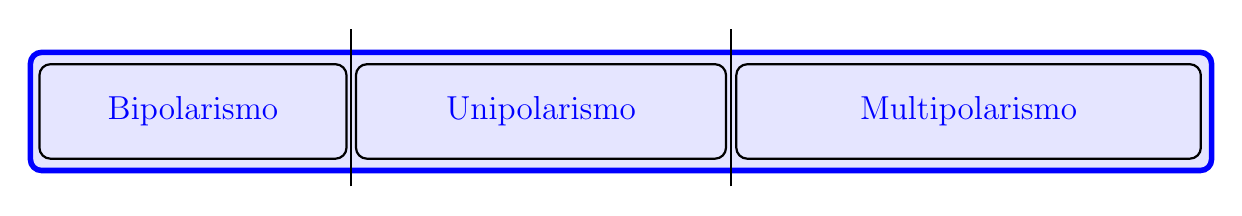
\begin{tikzpicture}
        \tikzset{box style/.style={draw, thick, rectangle, rounded corners, fill=blue!10, text=blue, font=\fontsize{12}{14}\selectfont}}
        \tikzset{line style/.style={line width=2pt, color=blue}}

        \draw[line style, fill=blue!10, rounded corners] (0,0) rectangle (15,1.5);
        \draw[thick] (4.075,-0.2) -- (4.075,1.8);
        \draw[thick] (8.9,-0.2) -- (8.9,1.8);

        \node[box style, anchor=west, minimum width=3.9cm, minimum height=1.2cm] at (0.1, 0.75) {Bipolarismo};
        \node[box style, anchor=west, minimum width=4.7cm, minimum height=1.2cm] at (4.12, 0.75) {Unipolarismo};
        \node[box style, anchor=west, minimum width=5.9cm, minimum height=1.2cm] at (8.95, 0.75) {Multipolarismo};
    \end{tikzpicture}

    %=== GRAFICO MULTILATERALISMO ===
    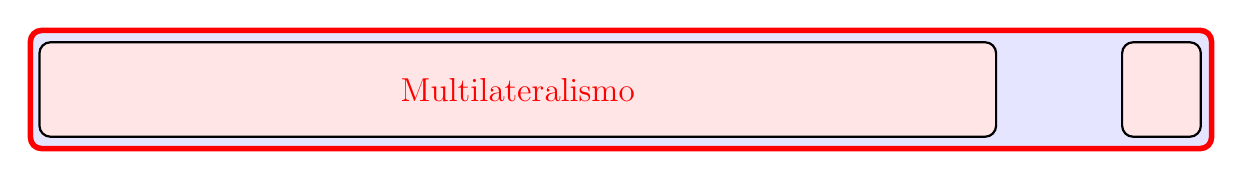
\begin{tikzpicture}
        \tikzset{box style/.style={draw, thick, rectangle, rounded corners, fill=red!10, text=red, font=\fontsize{12}{14}\selectfont}}
        \tikzset{line style/.style={line width=2pt, color=red}}

        \draw[line style, fill=blue!10, rounded corners] (0,0) rectangle (15,1.5);

        \node[box style, anchor=west, minimum width=12.15cm, minimum height=1.2cm] at (0.1, 0.75) {Multilateralismo};
        \node[box style, anchor=west, minimum width=1cm, minimum height=1.2cm] at (13.85, 0.75) {};
    \end{tikzpicture}
        %=== LINEA DEL TEMPO ===
    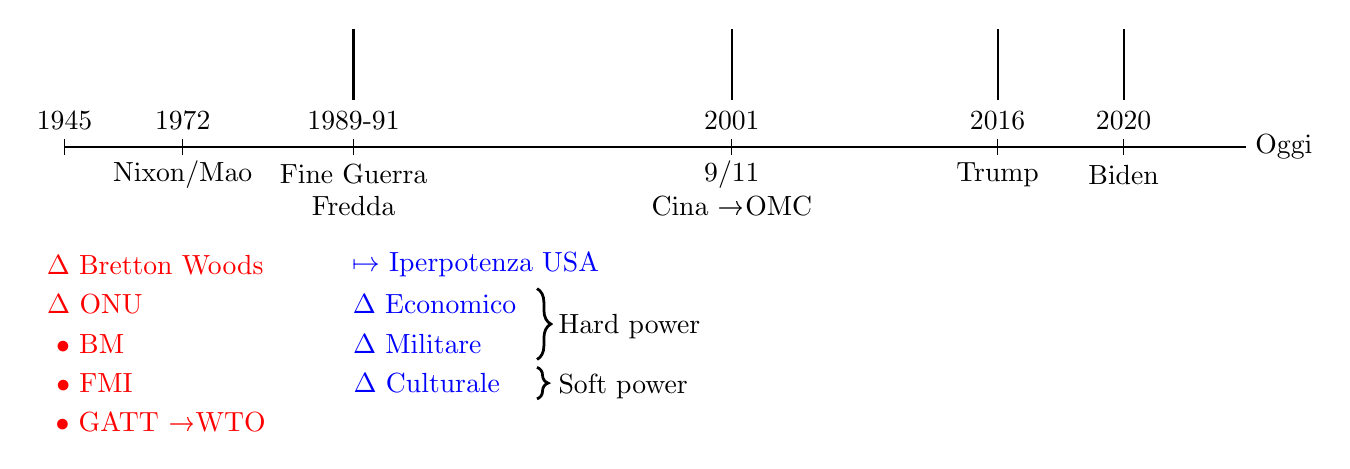
\begin{tikzpicture}
        \draw[thick] (0,0) -- (15,0);

        \foreach \x/\text in {0/1945, 1.5/1972, 3.67/1989-91, 8.475/2001, 11.85/2016, 13.45/2020}
            \draw (\x,-0.1) -- (\x,0.1) node[above] {\text};

        \node at (1.5,-0.35) {Nixon/Mao};
        \node at (3.67,-0.35) {Fine Guerra};
        \node at (3.67,-0.75) {Fredda};
        \draw[thick] (3.67,0.6) -- (3.67,1.5);
        \node at (8.475,-0.35) {9/11};
        \node at (8.475,-0.75) {Cina \textrightarrow OMC};
        \draw[thick] (8.475,0.6) -- (8.475,1.5);
        \node at (11.85,-0.35) {Trump};
        \draw[thick] (11.85,0.6) -- (11.85,1.5);
        \node at (13.45,-0.35) {Biden};
        \draw[thick] (13.45,0.6) -- (13.45,1.5);
        \node at (15,0) [right] {Oggi};

        %=== Legenda 1945 ===
        {\color{red}
        \node at (1.15,-1.5) {$\Delta$ Bretton Woods};
        \node at (0.385,-2) {$\Delta$ ONU};
        \node at (0.325,-2.5) {$\bullet$ BM};
        \node at (0.38,-3) {$\bullet$ FMI};
        \node at (1.22,-3.5) {$\bullet$ GATT \textrightarrow WTO};
        }

        %=== Legenda 1989 ===
        {\color{blue}
        \node at (5.22,-1.5) {$\mapsto$ Iperpotenza USA};
        \node at (4.7,-2) {$\Delta$ Economico};
        \node at (4.48,-2.5) {$\Delta$ Militare};
        \node at (4.6,-3) {$\Delta$ Culturale};
        }
        
        \draw[decorate, decoration={brace, amplitude=5pt, mirror}, line width=1pt] 
        (6,-2.7) -- (6,-1.8) node [black,midway,xshift=-0.6cm] {};
        \node[align=left, anchor=west] at (6.15, -2.28) {Hard power};

        \draw[decorate, decoration={brace, amplitude=4pt, mirror}, line width=1pt] 
        (6,-3.2) -- (6,-2.8) node [black,midway,xshift=-0.6cm] {};
        \node[align=left, anchor=west] at (6.15, -3.05) {Soft power};
    \end{tikzpicture}
\end{snippet}

\begin{snippet}{globalizzazione-lista-eventi}
    \textbf{Lista eventi:}
    \begin{itemize}
        \item Il bipolarismo conclude con la fine della Guerra fredda
            \begin{itemize}[label=\textrightarrow]
                \item 1989 - 1991: Dissoluzione dell'Unione Sovietica
                \item 1991 - 2001: Unipolarismo
            \end{itemize}
        \item Multilateralismo: Insieme di Stati e Nazioni che collaborano per un obiettivo comune
            \begin{itemize}[label=\textrightarrow]
                \item 09.11.2001: Crollo delle Torri Gemelle mostra gli USA come Stato vulnerabile:\\
                    Iperpotenza culturale {\color{red}{\circled{--}}}
                \item 2001: Cina entra nell'OMC\ \textrightarrow\ Stati Uniti non sono più i più forti
                    economicamente:\\ Iperpotenza economica {\color{red}{\circled{--}}}
                \item 2001 - 2008: G. W. Bush potenzia l'esercito statunitense (Guerra al Terrore):\\
                    Iperpotenza militare {\color{green}{\circled{+}}}
                \item 2007: Invasione dell'Iraq fa perdere molti uomini agli USA, influendo sulla soft power:\\
                    Iperpotenza militare e culturale {\color{red}{\circled{--}\circled{--}}}
            \end{itemize}
    \end{itemize}
\end{snippet}

\subsubsection{Globalizzazione e cambiamenti geopolitici}

\begin{snippet}{globalizzazione-e-cambiamenti-politici}
    Dopo la Seconda Guerra Mondiale, il mondo è passato da un equilibrio bipolare durante la Guerra
    fredda alla supremazia unipolare degli Stati Uniti seguendo il crollo dell'URSS.
    
    Questo cambio ha facilitato accordi economici transcontinentali come il NAFTA (North American Free Trade Agreemen)
    e l'espansione dell'APEC (Gruppo di cooperazione economica Asia-Pacifico), che hanno promosso la
    liberalizzazione del commercio e incrementato la cooperazione economica tra i continenti.
\end{snippet}

\subsubsection{Impatti sociali ed economici}

\begin{snippet}{impatti-sociali-ed-economici-globalizzazione}
    Nei decenni '80 e '90, l'indebitamento crescente nei paesi in via di sviluppo, aggravato da
    politiche monetarie restrittive come quelle degli Stati Uniti, ha portato a profonde crisi
    economiche.
    
    Le condizioni imposte dal FMI (Fondo Monetario Internazionale), come le riforme strutturali
    e le politiche di austerità, hanno spesso esacerbato le difficoltà economiche nei paesi in via
    di sviluppo, peggiorando la miseria e l'instabilità sociale.
\end{snippet}

\subsection{Nuovi attori e nuove visioni per la scena internazionale}

\subsubsection{Ascesa della Cina come superpotenza}

\begin{snippet}{globalizzazione-ascesa-cina-superpotenza}
    L'apertura diplomatica tra Stati Uniti e Cina, nel 1973, fu vista come una mossa che permise
    alla Cina di emergere come una superpotenza economica e politica, in grado di sfidare la
    supremazia americana e partecipare attivamente alla globalizzazione sotto l'egida degli Stati
    Uniti.
\end{snippet}

\subsubsection{Paesi di nuova industrializzazione (NIC)}

\begin{snippet}{globalizzazione-nic}
    Durante la fine degli anni '80 e l'inizio degli anni '90, alcuni paesi in Asia sudorientale,
    Africa australe e America Latina trasformarono le loro economie per adattarsi e partecipare ai
    grandi circuiti finanziari e commerciali globali.

    Accanto a questi paesi emergenti, vi furono paesi gravemente indebitati e paesi poveri con
    un'industrializzazione precaria e specializzati in poche materie prime. Queste nazioni
    riscontrarono difficoltà crescenti nel contesto globalizzato, evidenziando disparità nella
    distribuzione dei benefici della globalizzazione.
\end{snippet}

\subsubsection{Transizione dei paesi socialisti}

\begin{snippet}{globalizzazione-transizione-paesi-socialisti}
    Sempre nel periodo '80-'90, i paesi socialisti, compresi l'Unione Sovietica e gli stati
    dell'Europa centrale, lottarono per adattarsi al nuovo contesto economico globalizzato.
    Questo portò al crollo dell'URSS e alla dissoluzione del blocco socialista.

    Contrariamente ad altri paesi, la Cina mantenne il suo modello socialista, ma si aprì con
    prudenza alla globalizzazione, cercando di integrarsi senza rinunciare al controllo statale.

    L'integrazione di nuovi attori economici e la trasformazione dei paesi socialisti
    ristrutturarono significativamente il panorama geopolitico globale.
\end{snippet}

\end{document}